\section{Prodotti e servizi offerti}  
Eurosystem S.p.A. offre una gamma di prodotti e servizi informatici pensati per garantire la protezione delle infrastrutture \textit{IT} aziendali. In particolare, il reparto di \textit{cybersecurity} si occupa di diverse attività fondamentali per la difesa e la continuità operativa delle organizzazioni.\\\\  
Un primo ambito riguarda \textbf{il monitoraggio e la risposta agli incidenti}. Il \gls{soc}\glsadd{soc_def} e i servizi di \gls{mdr}\glsadd{mdr_def} assicurano un controllo costante delle reti aziendali, con l'obiettivo di rilevare in tempo reale anomalie e potenziali minacce. Il \textit{team} esamina ogni incidente nel dettaglio mediante la raccolta e l'analisi dei \textit{log} e dei dati di rete, l'identificazione dei vettori di attacco e delle vulnerabilità sfruttate, l'isolamento delle minacce e il ripristino dei sistemi tramite soluzioni di \textit{backup} e \textit{disaster recovery}. A completamento del processo, il \textit{team} redige \textit{report} dettagliati contenenti analisi, azioni intraprese e raccomandazioni di miglioramento.\\\\  
Un secondo ambito è rappresentato dalle \textbf{verifiche di sicurezza}, svolte tramite attività di \textit{Cyber Analysis Assessment}. In questa fase rientrano il \textit{Vulnerability Management} e i \textit{Penetration Test}, strumenti fondamentali per individuare e valutare i punti deboli delle infrastrutture \textit{IT}. A ciò si affiancano i servizi di \textit{Phishing Assessment}, utili a misurare la resilienza degli utenti contro campagne fraudolente, e le attività di \textit{Threat Intelligence}, finalizzate a raccogliere e analizzare informazioni utili a prevenire attacchi futuri.  
\begin{figure}[H]
    \centering
    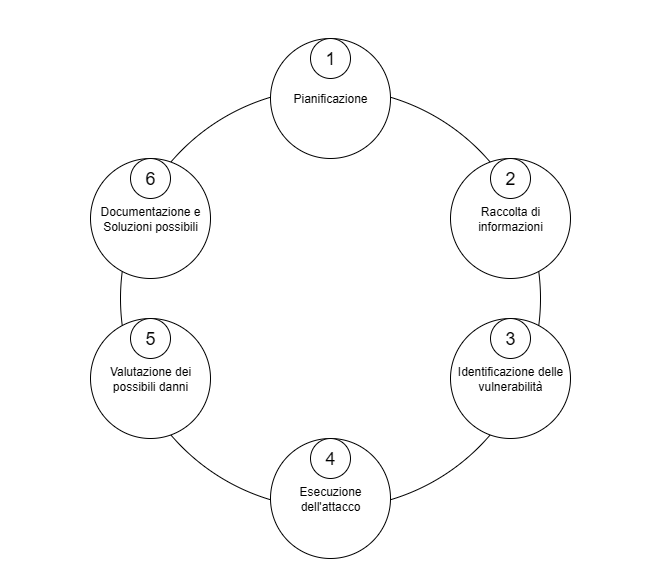
\includegraphics[alt={Schema Penetration Test}, width=0.95\columnwidth]{img/Pen_test.png}
    \caption{Schema di esempio di un processo di \textit{penetration testing}.}
    \label{fig:pen_test}    
\end{figure}  
\textbf{L'analisi delle reti} rappresenta un aspetto importante delle attività svolte. Questa comprende il monitoraggio del traffico di rete, il rilevamento di anomalie e la gestione degli eventi di sicurezza, con particolare attenzione alle reti industriali, al fine di contribuire alla continuità operativa dei processi produttivi.\\\\  
Un ruolo centrale è svolto anche dalla \textbf{gestione degli \textit{endpoint}}, ossia la protezione dei dispositivi aziendali, interni o remoti. Questa attività comprende il monitoraggio costante dello stato di sicurezza, l'applicazione degli aggiornamenti correttivi e delle politiche di protezione, il controllo delle identità e degli accessi, nonché il rilevamento e la risposta rapida alle minacce. Inoltre, sono previsti \textit{report} e \gls{audit} di conformità, volti a garantire trasparenza e allineamento con le normative.  
\begin{figure}[H]
    \centering
    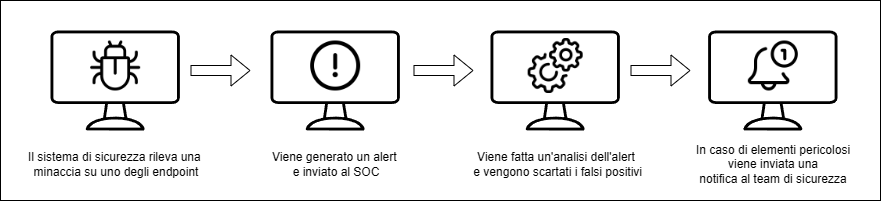
\includegraphics[alt={Schema Endpoint governance}, width=\columnwidth]{img/endpoint.png}
    \caption{Schema di esempio di un processo di gestione degli \textit{endpoint}.}
    \label{fig:endpoint_governance}    
\end{figure}  
Alla gestione degli \textit{endpoint} si affianca la \textbf{gestione dei dati}. Eurosystem S.p.A. supporta le aziende nella protezione, nell'organizzazione e nella conformità dei dati, in linea con i requisiti normativi, assicurando così un trattamento sicuro e affidabile delle informazioni.\\\\  
Un altro elemento di rilievo è la \textbf{gestione degli utenti e la sensibilizzazione}. L'azienda promuove attività formative mirate a diffondere buone pratiche di sicurezza informatica, con particolare attenzione agli accessi, ai privilegi e ai comportamenti corretti. In questo modo viene ridotto il rischio legato al fattore umano, spesso determinante nella riuscita di un attacco informatico.\\\\  
Infine, Eurosystem S.p.A. offre un \textbf{supporto tempestivo in caso di criticità}. In presenza di incidenti o sospette violazioni, i clienti ricevono un'assistenza diretta e immediata, con l'obiettivo di ridurre al minimo l'impatto sull'operatività aziendale.  
Grazie a questo insieme di attività, l'azienda è in grado di identificare proattivamente le vulnerabilità dei sistemi informativi, predisporre misure di protezione adeguate e garantire un aggiornamento costante delle competenze necessarie per affrontare l'evoluzione delle minacce informatiche.  
